\documentclass[10pt,twocolumn]{article}

% ---- packages (all in TeX Live) ----
\usepackage[margin=0.75in]{geometry}
\usepackage[T1]{fontenc}
\usepackage{lmodern}
\usepackage{microtype}
\usepackage{booktabs}
\usepackage{graphicx}
\usepackage{amsmath}
\usepackage{amssymb}
\usepackage{algorithm}
\usepackage[noend]{algpseudocode}
\usepackage{xcolor}
\usepackage{url}
\usepackage[colorlinks=true,linkcolor=blue,citecolor=blue,urlcolor=blue]{hyperref}
\usepackage[numbers,sort&compress]{natbib}
\usepackage{authblk}
\usepackage{caption}
\captionsetup{font=small}

\graphicspath{{figures/}}

\title{\vspace{-1.5em}Static Quantization as a Reproducibility Primitive\\ for Transformer Inference}
\author[1]{James Burrell}
\affil[1]{\normalsize \texttt{jburrell@tunnldata.com}}
\date{}

\begin{document}
\maketitle

\begin{abstract}
Floating-point Transformer inference is usually stable enough to deploy, but it
promises no bitwise equality across batch shapes, kernels, or hardware
platforms. We study whether \emph{static} weight-and-activation 8-bit
quantization (W8A8) should be understood as a \emph{reproducibility} mechanism
rather than only a compression or throughput mechanism. Using a frozen 286M
parameter NanoChat checkpoint, we run a preregistered matrix of seven arithmetic
methods across batch sizes 1, 8, and 64, with 1{,}000 greedy generations per
condition, and measure output multiplicity, match to an FP32 reference, logit
error, KL divergence, and held-out fidelity. We report three findings. First, a
\emph{null result}: on a single GPU, batch shape does not induce output
nondeterminism for any precision---greedy FP32 already matches its own batch-1
reference on 100\% of prompts, and every method is self-consistent across
process restarts. Second, a \emph{positive nuance}: integer matmul makes the
logits \emph{exactly} batch-invariant (maximum logit error identical to eight
significant figures across batch 1/8/64), which even FP32 is not; and this holds
for both static and dynamic scaling, so the mechanism is integer accumulation,
not scale freezing. Third, a \emph{tradeoff}: this invariance comes from
computing a \emph{different, lower-fidelity} function---static W8A8 matches the
FP32 reference on 0\% of prompts and raises validation bits-per-byte from 0.8395
to 0.8752. Finally, a CPU replication shows the invariance does \emph{not} extend
across platforms and in fact reverses: FP32 reproduces the same text on 100\% of
prompts across GPU and CPU, whereas static W8A8 reproduces only 25\%, because the
normalization, softmax, rotary, and dequantization operations remain floating
point and INT8 rounding sits near decision boundaries. We conclude that
quantization can deliver exact numerical batch-invariance \emph{within} a device
but, in this prototype, actively degrades cross-platform determinism, and we frame
integer-only NanoChat inference as the follow-on work.
\end{abstract}

\section{Introduction}
Practitioners routinely assume that a fixed model, checkpoint, and prompt yield a
fixed output. In floating point this assumption is false in a subtle way: the
IEEE-754 operations used by matrix multiplication are not associative, so the
order in which partial sums are accumulated---which depends on batch shape, the
kernel a library selects, and the hardware it runs on---can change the result at
the level of the last few bits~\cite{pytorch_numerical}. Those bits occasionally
propagate through an $\arg\max$ and change a generated token. Fixing a random
seed does not address this: seeding controls sampling, not the numerical path of
the forward pass~\cite{pytorch_reproducibility,he2025nondeterminism}.

Quantization is almost always motivated by memory and throughput. We take a
different position: an integer matmul accumulates in exact \texttt{int32}
arithmetic, so its result is \emph{independent} of accumulation order, and it is
therefore a natural candidate for a \emph{reproducibility primitive}. This paper
asks a narrow, measurable version of that question: \emph{does a fixed
quantization grid reduce a Transformer's output sensitivity to batch-shape
perturbation, relative to FP32, FP16, and BF16, and is any reduction attributable
to fixed scales or to the integer matmul itself?}

This is a position paper with a working prototype, not a completed integer-only
Transformer. Our prototype quantizes only the aligned core linear layers to
INT8$\times$INT8$\rightarrow$INT32 and dequantizes for every nonlinear and
residual operation; we use the label \textbf{static W8A8 linear} throughout to
keep that boundary explicit. Our contributions are:
\begin{itemize}\itemsep2pt
  \item A reframing of static quantization as a reproducibility mechanism, with
  operational definitions that separate determinism, repeatability, and fidelity.
  \item A NanoChat W8A8 prototype and a preregistered measurement protocol with
  deterministic-FP and dynamic-quantization controls.
  \item Controlled measurements showing (i) a same-machine null result, (ii)
  exact logit-level batch-invariance from integer matmul, (iii) a
  reproducibility/fidelity tradeoff, and (iv) a negative cross-platform result.
\end{itemize}

\section{Motivation and Problem Statement}
\paragraph{Definitions.} We distinguish four properties. \emph{Determinism}: the
same process, run twice, produces identical output. \emph{Repeatability}:
identical output across fresh process launches on the same machine.
\emph{Reproducibility}: identical output across batch shapes, kernels, or
platforms. \emph{Fidelity}: closeness of the output distribution to a chosen
FP32 reference. A method can be perfectly repeatable yet unfaithful, and this
distinction is central to our results.

\paragraph{Why batch shape matters.} A decode step for a single sequence and the
same step inside a batch of 64 traverse different kernels and reduction trees.
Because floating-point addition is non-associative, the resulting logits can
differ. Whether that difference changes a token is an empirical question, which
motivates our design: we hold the model, checkpoint, prompt, and decoding
schedule fixed and vary \emph{only} the physical batch shape and the arithmetic
method.

\paragraph{Research question.} Does calibration-fixed W8A8 linear inference reduce
NanoChat's numerical and generation sensitivity to batch shape and process
restart relative to floating point, and is any reduction attributable to fixed
scales rather than integer matrix multiplication alone? We do not equate fixed
seeds with deterministic inference, and we do not claim cross-platform
determinism from a single platform.

\section{Related Work}
\paragraph{Integer-only Transformers.} I-BERT~\cite{kim2021ibert} approximates
GELU, softmax, and layer normalization with integer and dyadic arithmetic so
that BERT inference is integer-only. I-ViT~\cite{li2023ivit} extends this to
vision Transformers with integer attention and normalization. These works target
accuracy and latency; they establish that the nonlinear operations we leave in
floating point \emph{can} be made integer, which is precisely our roadmap.

\paragraph{LLM post-training quantization.} LLM.int8()~\cite{dettmers2022llmint8}
and SmoothQuant~\cite{xiao2023smoothquant} make W8A8 accurate at scale by
handling activation outliers, and the integer-arithmetic training of
\citet{jacob2018quantization} underpins modern W8A8. This literature optimizes
accuracy, memory, and throughput. To our knowledge it does not measure
\emph{generation reproducibility} as the primary outcome.

\paragraph{Cross-platform consistency and framework guidance.} Cross-platform
post-training quantization has been studied where encoder/decoder mismatch is
catastrophic, e.g.\ learned image compression~\cite{yu2022crossplatform}. Vendor
documentation warns that batched and sliced computations need not be bitwise
equal and that determinism requires explicit, performance-costly
flags~\cite{pytorch_numerical,pytorch_reproducibility}. Recent systems work makes
LLM inference batch-invariant by controlling reductions~\cite{he2025nondeterminism};
we ask whether quantization achieves a similar invariance as a side effect of
integer accumulation, and at what fidelity cost. The gap we address: most
quantization work treats reproducibility as incidental rather than as the
measured objective.

\section{NanoChat W8A8 Prototype}
\paragraph{Model.} We use a frozen NanoChat~\cite{karpathy2025nanochat} base
checkpoint (\texttt{paper-d12}, step 2520; 12 layers, $d{=}768$, 6 heads,
vocabulary 32768; 286{,}261{,}730 parameters; trained on 1.321B tokens; validation
BPB 0.8396). The checkpoint, tokenizer, and prompt/calibration manifests are
pinned by SHA-256 and archived with every result directory.

\paragraph{Arithmetic conditions.} \emph{FP32} is literal float32 with TF32
disabled. \emph{FP16} and \emph{BF16} use NanoChat's explicit half-precision
compute paths. Deterministic FP32/FP16 controls enable PyTorch deterministic
algorithms with a fixed cuBLAS workspace. The \emph{static W8A8} prototype uses
symmetric INT8 with per-output-channel weight scales and a per-tensor activation
scale frozen from 32 calibration strings; it executes
INT8$\times$INT8$\rightarrow$INT32 with PyTorch's \texttt{\_int\_mm} and
dequantizes the \texttt{int32} accumulator. The \emph{dynamic W8A8} control uses
the identical integer matmul but re-estimates the activation scale at runtime;
comparing the two isolates whether any stability comes from the fixed grid or
from integer arithmetic alone.

\begin{algorithm}[t]
\caption{Static W8A8 linear (per-channel weights, per-tensor frozen activation).}
\label{alg:w8a8}
\footnotesize
\begin{algorithmic}[1]
\State \textbf{Calibrate:} run the float model on 32 calibration strings; for each
eligible linear record $a^{\star}\!=\!\max|x|$ over its observed inputs.
\State \textbf{Freeze weights:} $s_w \gets \max_{\text{col}}|W| / 127$;\;
$W_q \gets \mathrm{clip}(\mathrm{round}(W / s_w), -127, 127)$
\State \textbf{Freeze activation scale:} $s_a \gets a^{\star} / 127$
\Statex \textbf{Forward}$(x)$:
\State $x_q \gets \mathrm{clip}(\mathrm{round}(x / s_a), -127, 127)$ \Comment{INT8}
\State \textbf{if} rows$(x_q)<32$ \textbf{then} zero-pad to 32 rows \Comment{\texttt{\_int\_mm}}
\State $A \gets \texttt{\_int\_mm}(x_q, W_q^\top)$ \Comment{exact INT32 accumulation}
\State \Return $A_{[:\text{rows}]} \cdot (s_a s_w) + b$ \Comment{dequantize in FP}
\end{algorithmic}
\end{algorithm}

\paragraph{Claim boundary.} Only aligned core projections are quantized
(in/out features divisible by 8). NanoChat's tiny unaligned smear and value-gate
projections, and all normalization, rotary embedding, attention softmax,
residual, and dequantization operations, remain floating point. This isolates
grid snapping and integer accumulation but is \emph{not} integer-only inference.
For decode matmuls with 16 or fewer rows---which PyTorch's CUDA \texttt{\_int\_mm}
rejects---both W8A8 paths zero-pad to 32 rows and slice the padding from the
output; this shared compatibility path is reported in the limitations.

\section{Experimental Protocol}
The protocol is preregistered and frozen. For every arithmetic
method\,$\times$\,batch size $\in\{1,8,64\}$ we retain exactly 1{,}000 greedy
generations: 20 prompts $\times$ 10 replicas $\times$ 5 fresh process launches.
The final partial logical batch is padded to the declared physical batch size and
padding rows are discarded, so every launch uses the stated shape. The FP32
batch-1 teacher-forced trace is the common reference. A fixed-sample secondary
experiment uses pre-generated CPU uniforms shared by every replica to avoid
batch-dependent RNG consumption.

\paragraph{Outcomes.} Generation: unique sequences per prompt across restarts,
FP32 batch-1 reference-match rate, and modal fraction. Numerical: mean and
maximum absolute logit difference, logit RMSE, and forward KL from the FP32
batch-1 distribution. Fidelity: held-out validation BPB over 2{,}097{,}152 tokens,
throughput, and a static calibration-size sensitivity at 1/8/32 samples.

\paragraph{Statistics.} We report prompt-level means and 95\% prompt-cluster
bootstrap intervals (10{,}000 resamples, seed 20260621). Replicas and process
launches are repeated measurements, not independent prompts. Every prespecified
condition is reported, including null results. Hardware/software versions, Git
state, and device queries are archived per run.

\paragraph{Hypotheses.} \textbf{H1} (sanity): FP16 deviates from the FP32 batch-1
reference more than FP32 does at batch 8/64. \textbf{H2} (central): static W8A8
has lower within-condition output multiplicity than FP16 under batch
perturbation. \textbf{H3}: static W8A8 may raise reference-match rate while
increasing KL, separating reproducibility from fidelity. \textbf{H4}: static is
more stable than dynamic W8A8 if scale freezing, rather than integer matmul, is
the mechanism.

\section{Results}
Table~\ref{tab:main} reports the greedy matrix; Figures~\ref{fig:match}--%
\ref{fig:logit} visualize the key columns, and Table~\ref{tab:fidelity} the
fidelity ablation.

\begin{table}[t]
\centering
\caption{Greedy matrix (1{,}000 generations per row). $|\Delta|$ is absolute
logit difference from the FP32 batch-1 reference; KL is forward KL in nats; BPB
is held-out validation fidelity. Static/dynamic W8A8 use calibration 32.}
\label{tab:main}
\footnotesize
\setlength{\tabcolsep}{3.5pt}
\begin{tabular}{llrrrrr}
\toprule
Method & Batch & Match & Mean$|\Delta|$ & Max$|\Delta|$ & KL & BPB \\
\midrule
FP32 & 1 & 1.00 & 0.00e+00 & 0.00e+00 & 2.18e-09 & 0.8395 \\
FP32 & 8 & 1.00 & 1.08e-06 & 1.32e-05 & 2.29e-09 & 0.8395 \\
FP32 & 64 & 1.00 & 1.74e-06 & 1.62e-05 & 5.23e-09 & 0.8395 \\
\addlinespace
FP16 & 1 & 0.95 & 3.22e-03 & 2.34e-02 & 2.31e-06 & 0.8395 \\
FP16 & 8 & 0.95 & 3.21e-03 & 2.33e-02 & 2.33e-06 & 0.8395 \\
FP16 & 64 & 0.95 & 3.19e-03 & 2.42e-02 & 2.33e-06 & 0.8395 \\
\addlinespace
BF16 & 1 & 0.75 & 2.56e-02 & 1.83e-01 & 1.46e-04 & 0.8396 \\
BF16 & 8 & 0.70 & 2.56e-02 & 1.80e-01 & 1.46e-04 & 0.8396 \\
BF16 & 64 & 0.70 & 2.57e-02 & 1.85e-01 & 1.47e-04 & 0.8396 \\
\addlinespace
Static W8A8 & 1 & 0.00 & 6.92e-01 & 4.88e+00 & 9.55e-02 & 0.8752 \\
Static W8A8 & 8 & 0.00 & 6.92e-01 & 4.88e+00 & 9.55e-02 & 0.8752 \\
Static W8A8 & 64 & 0.00 & 6.92e-01 & 4.88e+00 & 9.55e-02 & 0.8752 \\
\addlinespace
Dynamic W8A8 & 1 & 0.15 & 3.52e-01 & 3.48e+00 & 3.42e-02 & 0.8761 \\
Dynamic W8A8 & 8 & 0.15 & 3.52e-01 & 3.48e+00 & 3.40e-02 & 0.8761 \\
Dynamic W8A8 & 64 & 0.15 & 3.52e-01 & 3.48e+00 & 3.40e-02 & 0.8761 \\
\addlinespace
\bottomrule
\end{tabular}

\end{table}

\paragraph{A same-machine null result (H1, H2).} On one GPU, batch shape induces
\emph{no} output nondeterminism. Every method at every batch size has unique
output count 1.0: each prompt yields a single sequence across all replicas and
process launches. FP32 matches its own batch-1 reference on 100\% of prompts at
batch 8 and 64, despite a nonzero maximum logit drift of $\sim\!1.6\times10^{-5}$;
that drift never crosses an $\arg\max$ boundary. H1 holds directionally---FP16
($|\Delta|_{\max}\!\approx\!0.024$) and BF16 ($\approx\!0.18$) deviate far more
than FP32---but H2 finds \emph{no multiplicity to reduce}: FP16 and BF16 are
already output-deterministic across batch on this machine. The motivating
instability, at the level of emitted tokens, does not appear same-machine.

\begin{figure}[t]
\centering
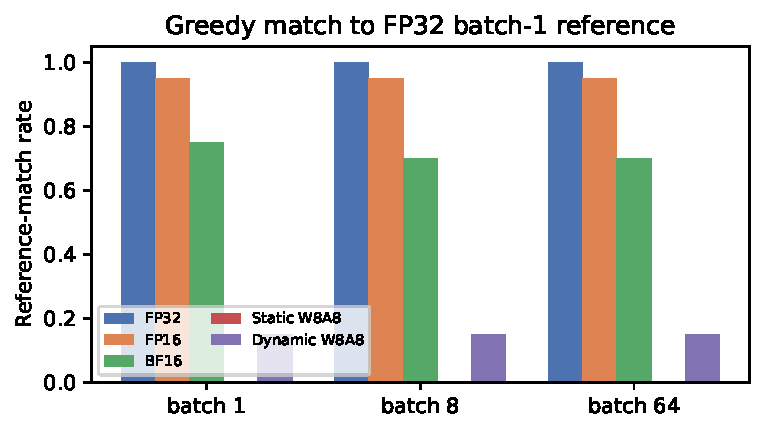
\includegraphics[width=\linewidth]{fig1_match_rate.pdf}
\caption{Reference-match rate to the FP32 batch-1 greedy reference. FP32 is exact;
FP16/BF16 flip a stable minority of tokens; W8A8 computes a different function.}
\label{fig:match}
\end{figure}

\paragraph{Exact batch-invariance from integer matmul (nuance).} Where floats
carry small batch-dependent noise, the integer paths do not. Static W8A8's maximum
logit error is \texttt{4.879709410667419} at batch 1, 8, \emph{and} 64---identical
to eight significant figures (Table~\ref{tab:main}, Fig.~\ref{fig:logit})---so its
logits are exactly invariant to batch shape, which FP32 is not. Dynamic W8A8 is
likewise invariant (\texttt{3.48} across all batches). Because both the fixed-scale
and the runtime-scale variants are exactly invariant, \textbf{H4 is not
supported}: the reproducibility mechanism is exact integer accumulation, not scale
freezing. Scale freezing instead affects \emph{fidelity} (below).

\begin{figure}[t]
\centering
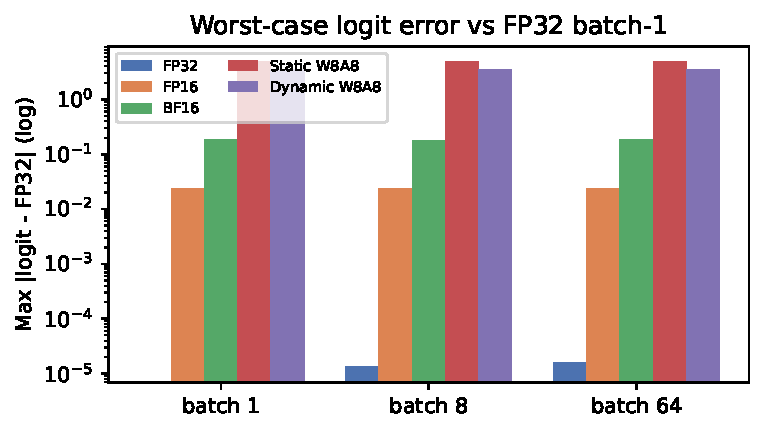
\includegraphics[width=\linewidth]{fig3_logit_error.pdf}
\caption{Worst-case logit error vs.\ FP32 batch-1 (log scale). FP32 batch-1 is
zero by construction; float error grows slightly with batch, while W8A8 error is
large but \emph{constant} across batch shape.}
\label{fig:logit}
\end{figure}

\paragraph{Reproducibility is not fidelity (H3).} The invariance is purchased by
computing a different function. Static W8A8 matches the FP32 reference on 0\% of
prompts and dynamic on 15\%; static W8A8's mean KL from FP32 is 0.095 nats versus
$2.3\times10^{-6}$ for FP16. Fidelity degrades accordingly: validation BPB rises
from 0.8395 (FP32) to 0.8752 (static W8A8) and 0.8761 (dynamic), whereas FP16 and
BF16 stay within $10^{-4}$ of FP32 (Table~\ref{tab:fidelity},
Fig.~\ref{fig:kl}). H3 is confirmed in its strong form: a W8A8 model can be
perfectly repeatable and batch-invariant while being a measurably worse
approximation of FP32. Static calibration size has a second-order effect (BPB
0.8771/0.8751/0.8752 at 1/8/32 samples), so 8 calibration strings already
saturate the fixed grid.

\begin{figure}[t]
\centering
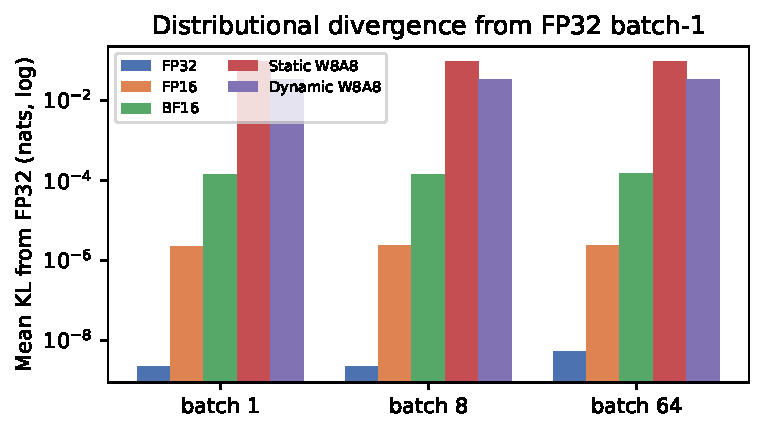
\includegraphics[width=\linewidth]{fig2_kl.pdf}
\caption{Mean forward KL from FP32 batch-1 (log scale). The integer paths trade
four to five orders of magnitude of divergence for exact batch-invariance.}
\label{fig:kl}
\end{figure}

\paragraph{Where precision flips tokens.} Reproducibility risk is
content-dependent (Table~\ref{tab:categories}). Under FP16 and BF16, factual,
numerical, reasoning, and instruction prompts match the FP32 reference on 100\% of
cases, while \emph{completion} and \emph{ambiguous} prompts flip most often (BF16
matches on only 33\% of each). These are prompts whose top logits are nearly tied,
so a $10^{-2}$-scale perturbation crosses the decision boundary; well-determined
prompts are unaffected. The static W8A8 column is uniformly zero because it
computes a different function on every prompt, not because ambiguity drives its
disagreement. With three prompts per category this is a descriptive signal, not a
powered test, but it indicates that any deployment-time reproducibility budget
should be spent on open-ended generation rather than factual recall.

\begin{table}[t]
\centering
\caption{Per-category reference-match rate (batch 1). Lower means the precision
flips more tokens relative to FP32. Completion/ambiguous prompts are most fragile.}
\label{tab:categories}
\footnotesize
\setlength{\tabcolsep}{3pt}
\begin{tabular}{lrrrr}
\toprule
Category & FP16 & BF16 & Static W8A8 & Dynamic W8A8 \\
\midrule
Factual & 1.00 & 1.00 & 0.00 & 0.00 \\
Reasoning & 1.00 & 1.00 & 0.00 & 0.33 \\
Numerical & 1.00 & 1.00 & 0.00 & 0.50 \\
Technical & 1.00 & 0.67 & 0.00 & 0.00 \\
Instruction & 1.00 & 1.00 & 0.00 & 0.00 \\
Completion & 0.67 & 0.33 & 0.00 & 0.00 \\
Ambiguous & 1.00 & 0.33 & 0.00 & 0.33 \\
\bottomrule
\end{tabular}

\end{table}

\begin{table}[t]
\centering
\caption{Fidelity ablation: held-out validation BPB over 2.1M tokens.}
\label{tab:fidelity}
\footnotesize
\begin{tabular}{llr}
\toprule
Method & Calib.\ samples & Validation BPB \\
\midrule
BF16 & -- & 0.83959 \\
Dynamic W8A8 & -- & 0.87612 \\
FP16 & -- & 0.83954 \\
FP32 & -- & 0.83954 \\
Static W8A8 & 1 & 0.87715 \\
Static W8A8 & 8 & 0.87509 \\
Static W8A8 & 32 & 0.87520 \\
\bottomrule
\end{tabular}

\end{table}

\paragraph{Cross-platform replication (CPU).} To test whether integer-matmul
invariance extends beyond one device, we replicate the core methods on a CPU
platform, where \texttt{\_int\_mm} executes but every surrounding operation uses
entirely different kernels and reduction orders. We measure the cleanest
cross-platform outcome available---whether the modal generated \emph{token
sequence} for each prompt is identical on GPU and CPU---so the comparison needs no
logit alignment. Table~\ref{tab:crossplatform} and Fig.~\ref{fig:crossplatform}
report the result, and it is the opposite of the naive expectation. FP32
reproduces the same text on \textbf{100\%} of prompts across platforms: at full
precision the GPU$\leftrightarrow$CPU logit gap never crosses an $\arg\max$
boundary. Agreement then \emph{falls} as precision drops---BF16 85\%, dynamic W8A8
45\%, and static W8A8 only \textbf{25\%}. Quantization is thus markedly
\emph{worse} for cross-platform reproducibility than full precision, not better.
The mechanism is consistent with our within-platform findings: integer
accumulation removes \emph{batch}-dependent variation, but INT8 rounding places
many logits near decision boundaries, and the surrounding floating-point
operations---dequantization, normalization, softmax, rotary embeddings---use
different kernels and reduction orders on CPU than on GPU. Those two effects
compound, so the integer paths flip far more tokens across platforms than FP32
does. This is the central negative result of the paper: exact batch-invariance
within a device does \emph{not} imply determinism across devices, and in this
prototype quantization actively degrades it.

\begin{table}[t]
\centering
\caption{Cross-platform replication: fraction of prompts whose modal greedy token
sequence is identical on GPU and CPU (batch 1).}
\label{tab:crossplatform}
\footnotesize
\begin{tabular}{lr}
\toprule
Method & GPU$\leftrightarrow$CPU text match \\
\midrule
FP32 & 100.0\% \\
BF16 & 85.0\% \\
Static W8A8 & 25.0\% \\
Dynamic W8A8 & 45.0\% \\
\bottomrule
\end{tabular}

\end{table}

\begin{figure}[t]
\centering
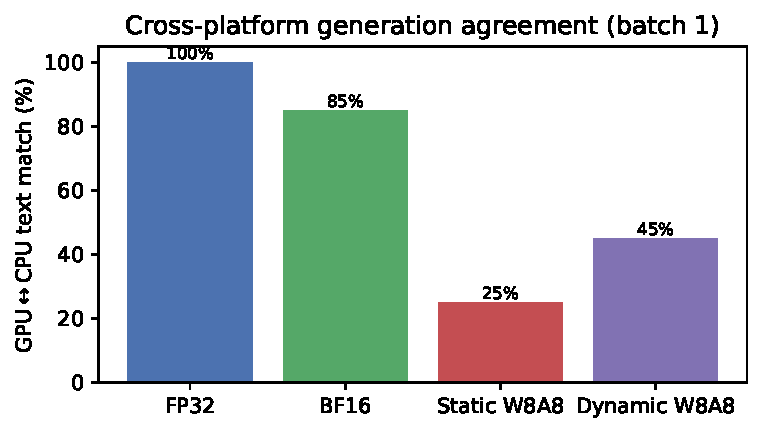
\includegraphics[width=\linewidth]{fig5_crossplatform.pdf}
\caption{GPU$\leftrightarrow$CPU generation agreement. Full precision is already
platform-stable at the token level; lower precision diverges. The integer paths'
remaining floating-point operations prevent bitwise platform invariance.}
\label{fig:crossplatform}
\end{figure}

\section{Discussion, Threats, and Roadmap}
\paragraph{A null result is informative.} For this model on this GPU, greedy
same-machine inference is already batch-invariant at the token level; the
reproducibility problem practitioners fear does not manifest here as output
divergence. Quantization is therefore \emph{not} needed to stabilize
same-machine batching, and using it for that purpose would forfeit fidelity for no
reproducibility gain. The defensible positive claim is narrower and exact:
integer matmul yields bitwise-identical logits across batch shapes, which matters
for applications that compare log-probabilities or require reproducible scoring
rather than merely reproducible tokens.

\paragraph{Threats to validity.} (i) One model, one checkpoint, and two devices
cannot establish generality. (ii) Batch shape changes tensor shapes but does not
cover kernel-library or driver drift, which cross-platform work must address.
(iii) Quantization error (KL 0.095) vastly exceeds the floating-point differences
it suppresses ($\text{KL}\!\approx\!10^{-9}$ for FP32 across batch), so the
``cure'' is larger than the ``disease'' unless downstream use is tolerant. (iv)
Our prototype quantizes only aligned linears; the padding compatibility path and
the remaining float operations are confounds for any strict determinism claim.

\paragraph{Roadmap.} The findings point to a clear next step: replace the
floating-point islands---integer softmax and RMSNorm following
I-BERT/I-ViT~\cite{kim2021ibert,li2023ivit}, fixed-point rotary tables, and an
integer residual path---so that batch-invariance can become platform-invariance.
Completing the cross-GPU/CPU replication, adding a fixed-sample secondary sweep,
and a downstream quality evaluation would let the reproducibility claim be stated
without the fidelity caveats we currently must attach.

\section{Conclusion}
Studied as a reproducibility primitive rather than a compression trick, static
W8A8 delivers exactly what integer accumulation promises---logits invariant to
batch shape---but no more: it is a different, lower-fidelity function, and its
invariance not only fails to survive a change of hardware platform but reverses,
dropping cross-platform text agreement from 100\% (FP32) to 25\% because most of
the network is still floating point and INT8 logits sit near decision boundaries.
On a single modern GPU, greedy inference is already batch-invariant at the token
level, so the value of quantization here is exact numerical, not behavioral,
reproducibility. The clear lesson is that batch-invariance and platform-invariance
are distinct goals, and only the former follows from integer matmul alone.
Full integer-only NanoChat inference---replacing the remaining floating-point
islands so that batch-invariance can extend to cross-platform determinism---is the
natural follow-on work.

{\footnotesize
\paragraph{Reproducibility.} All checkpoints, manifests, per-condition JSON,
figures, and the analysis scripts that regenerate every table and figure are
archived with the paper.}

\bibliographystyle{plainnat}
\bibliography{references}

\end{document}
